\chapter {Nagios}

\textbf{Nagios Core} é uma ferramenta de monitorização de sistemas grátis e \textit{open-source} \cite{Nagios}.
É também oferecido um serviço pago Nagios XI, que é construído sobre o sistema \textit{core}.

Esta ferramenta permite a monitorização de vários serviços, atuando como um \textit{scheduler} que executa periodicamente testes para verificar o estado dos serviços e sistemas.
Estes testes são os \textbf{plugins}, \textit{scripts} maioritariamente Perl, executáveis, desenvolvidos quer internamente, quer pela comunidade.
Existem plugins para testar várias funcionalidades, desde o estado de um servidor HTTP à carga de utilização do CPU num servidor.

É disponibilizada uma interface Web, com recurso ao Apache, onde várias estatísticas são apresentadas para o utilizador, assim como alertas sobre sistemas que estejam \textit{down}.
É de notar que várias versões do \textit{frontend} são disponibilizadas, aumentando a capacidade de customização do sistema.

Todas as configurações são feitas através de ficheiros \textit{txt} no host do Nagios, pelo que não é possível configurar a ferramenta na sua interface Web.

\begin{figure}[H]
    \centering
    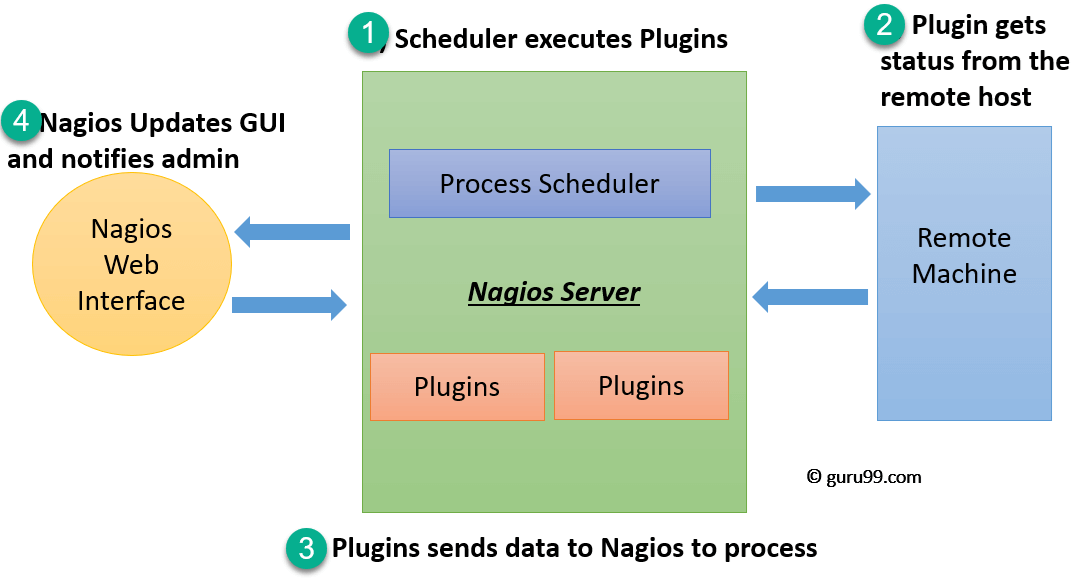
\includegraphics[width=.8\linewidth]{figs/nagios/nagios_wp}
    \caption{Princípio de funcionamento do Nagios}
    \label{fig:nagios_wp}
\end{figure}

\pagebreak

\section{Instalação e configuração}

A instalação foi feita segundo o guia de instalação do próprio Nagios \cite{Nagios_setup} no Tux13.
Foram definidos os dados de autenticação com o utilizador default \textit{nagiosadmin}.

Após a configuração inicial, foi feita a configuração dos sistemas.

O primeiro passo é importar os \textbf{Plugins} do Nagios.
Os seguintes \textit{packages} foram instalados no servidor:

\begin{itemize}
    \item nagios-plugins: os testes executáveis locais, i.e., que testam os serviços acedendo remotamente, por exemplo, a um servidor HTTP para verificar se está disponível.
    \item nagios-nrpe-plugins: os testes executáveis dos agentes, i.e., que são executados no sistema de destino para ter acesso a informação local, por exemplo, da utilização do CPU.
\end{itemize}

Devido aos objetivos deste trabalho consistirem maioritariamente com o teste dos serviços, foi utilizada a abordagem mais simples dos \textbf{nagios-plugins},
que não requer a instalação de agentes no computadores, apenas no servidor.

O segundo passo consiste em indicar ao Nagios quais os plugins utilizar e em que sistemas.
Para efeitos de simplificação, foi criada a pasta \verb|servers| no diretório \verb|/usr/local/nagios/etc/servers|.
Nesta pasta, foi criado um ficheiro .cfg para cada sistema, neste caso, \verb|tux12.cfg, localhost.cfg, tux13.cfg, router.cfg e switch.cfg|.

Nestes ficheiros é especificado quais são os plugins a executar em cada um dos computadores.
Por exemplo, o ficheiro \verb|tux12.cfg| ficou configurado da seguinte forma:

\pagebreak

\begin{lstlisting}
define host {
        use                          linux-server
        host_name                    tux12
        alias                        FTP-NTP-Mail
        address                      172.16.1.12
        register                     1
}

define service {

        use                     generic-service
        host_name               tux12
        service_description     Mail
        check_command           check_smtp
        notifications_enabled   1
}

define service {

        use                     generic-service
        host_name               tux12
        service_description     Ping
        check_command           check_ping
        notifications_enabled   1
}

define service {

        use                     generic-service
        host_name               tux12
        service_description     FTP
        check_command           check_ftp
        notifications_enabled   1
}
define service {

        use                     generic-service
        host_name               tux12
        service_description     NTP
        check_command           check_ntp_time
        notifications_enabled   1
}

define service {

        use                     generic-service
        host_name               tux12
        service_description     SSH
        check_command           check_ssh
}

\end{lstlisting}

Note-se que primeiro é feita uma definição do host e do respetivo IP.
Nos serviços, são identificados os testes a ser executados, especificando o host.
É possível definir todos os testes e hosts no mesmo ficheiro, mas tal não é boa prática pois torna-se muito difícil modificar as configurações do sistema.

\pagebreak

Dependendo do host e os serviços nele alojados, diferentes testes foram configurados:

\begin{table}[H]
    \begin{center}
        \begin{tabular}{ || c | c ||}
        \hline
        \textbf{Sistema} & \textbf{Testes}\\ 
        \hline
        Tux12 & \begin{tabular}{@{}c@{}}check\_ping \\ check\_ssh \\ check\_ntp \\ check\_ftp \\ check\_smtp (Mail)\end{tabular}\\
        \hline
        Tux14 & \begin{tabular}{@{}c@{}}check\_ping \\ check\_ssh \\ check\_http \\ check\_dns \\ check\_smtp (Mail)\end{tabular}\\
        \hline
        Router & \begin{tabular}{@{}c@{}}check\_ping \\ check\_snmp\_uptime\_v2 \\ \end{tabular}\\
        \hline
        Switch & \begin{tabular}{@{}c@{}}check\_ping \\ check\_snmp\_uptime\_v2 \\ \end{tabular}\\
        \hline
        Tux13 & localhost default tests \\
        \hline
        
        \end{tabular}
    \end{center}    
    \caption{Alocação dos serviços nos computadores}
    \label{tab:check_table}
\end{table}

Dois testes requereram mais atenção.

\textbf{Check\_dns}, apesar de ser um plugin instalado no \textit{package}, não está configurado no ficheiro \verb|commands.cfg|.
Este ficheiro é onde se define a sintax para correr os testes. Muitos já estão configurados, mas este não.
Desse modo configurou-se do seguinte modo:

\begin{lstlisting}

define command {
    command_name    check_dns
    command_line    $USER1$/check_dns -H $ARG1$ -s $HOSTADDRESS$ -a $ARG2$
}
\end{lstlisting}

com -H o endereço a fazer a \textit{query}, -s o servidor DNS a usar e -a o endereço IP esperado.
Os argumentos são passados quando se define o teste nos ficheiros de configuração.

\pagebreak

O teste predefinido do snmp, \textbf{check\_snmp}, não funcionou, pelo que instalou manualmente um novo script \textbf{check\_uptime} \footnote{\url{https://exchange.nagios.org/directory/Plugins/System-Metrics/Uptime/check_uptime--2F-check_snmp_uptime/details}}para o mesmo efeito.
Este script Perl for importado para a pasta \verb|\usr\lib\nagios\plugins|, sendo posteriormente definido como um executável para funcionar corretamente.
Este foi configurado do seguinte modo no ficheiro \verb|commands.cfg|:

\begin{lstlisting}

    define command {
        command_name check_snmp_uptime_v2
        command_line $USER1$/check_uptime.pl -2 -f -w -H $HOSTADDRESS$ -C public -T unix-sys
    }
\end{lstlisting}

Este comando retorna o OID \textbf{sysUpTime} do SNMP no sistema, verificando assim o seu funcionamento.

\section{Resultados}

\begin{figure}[H]
    \centering
    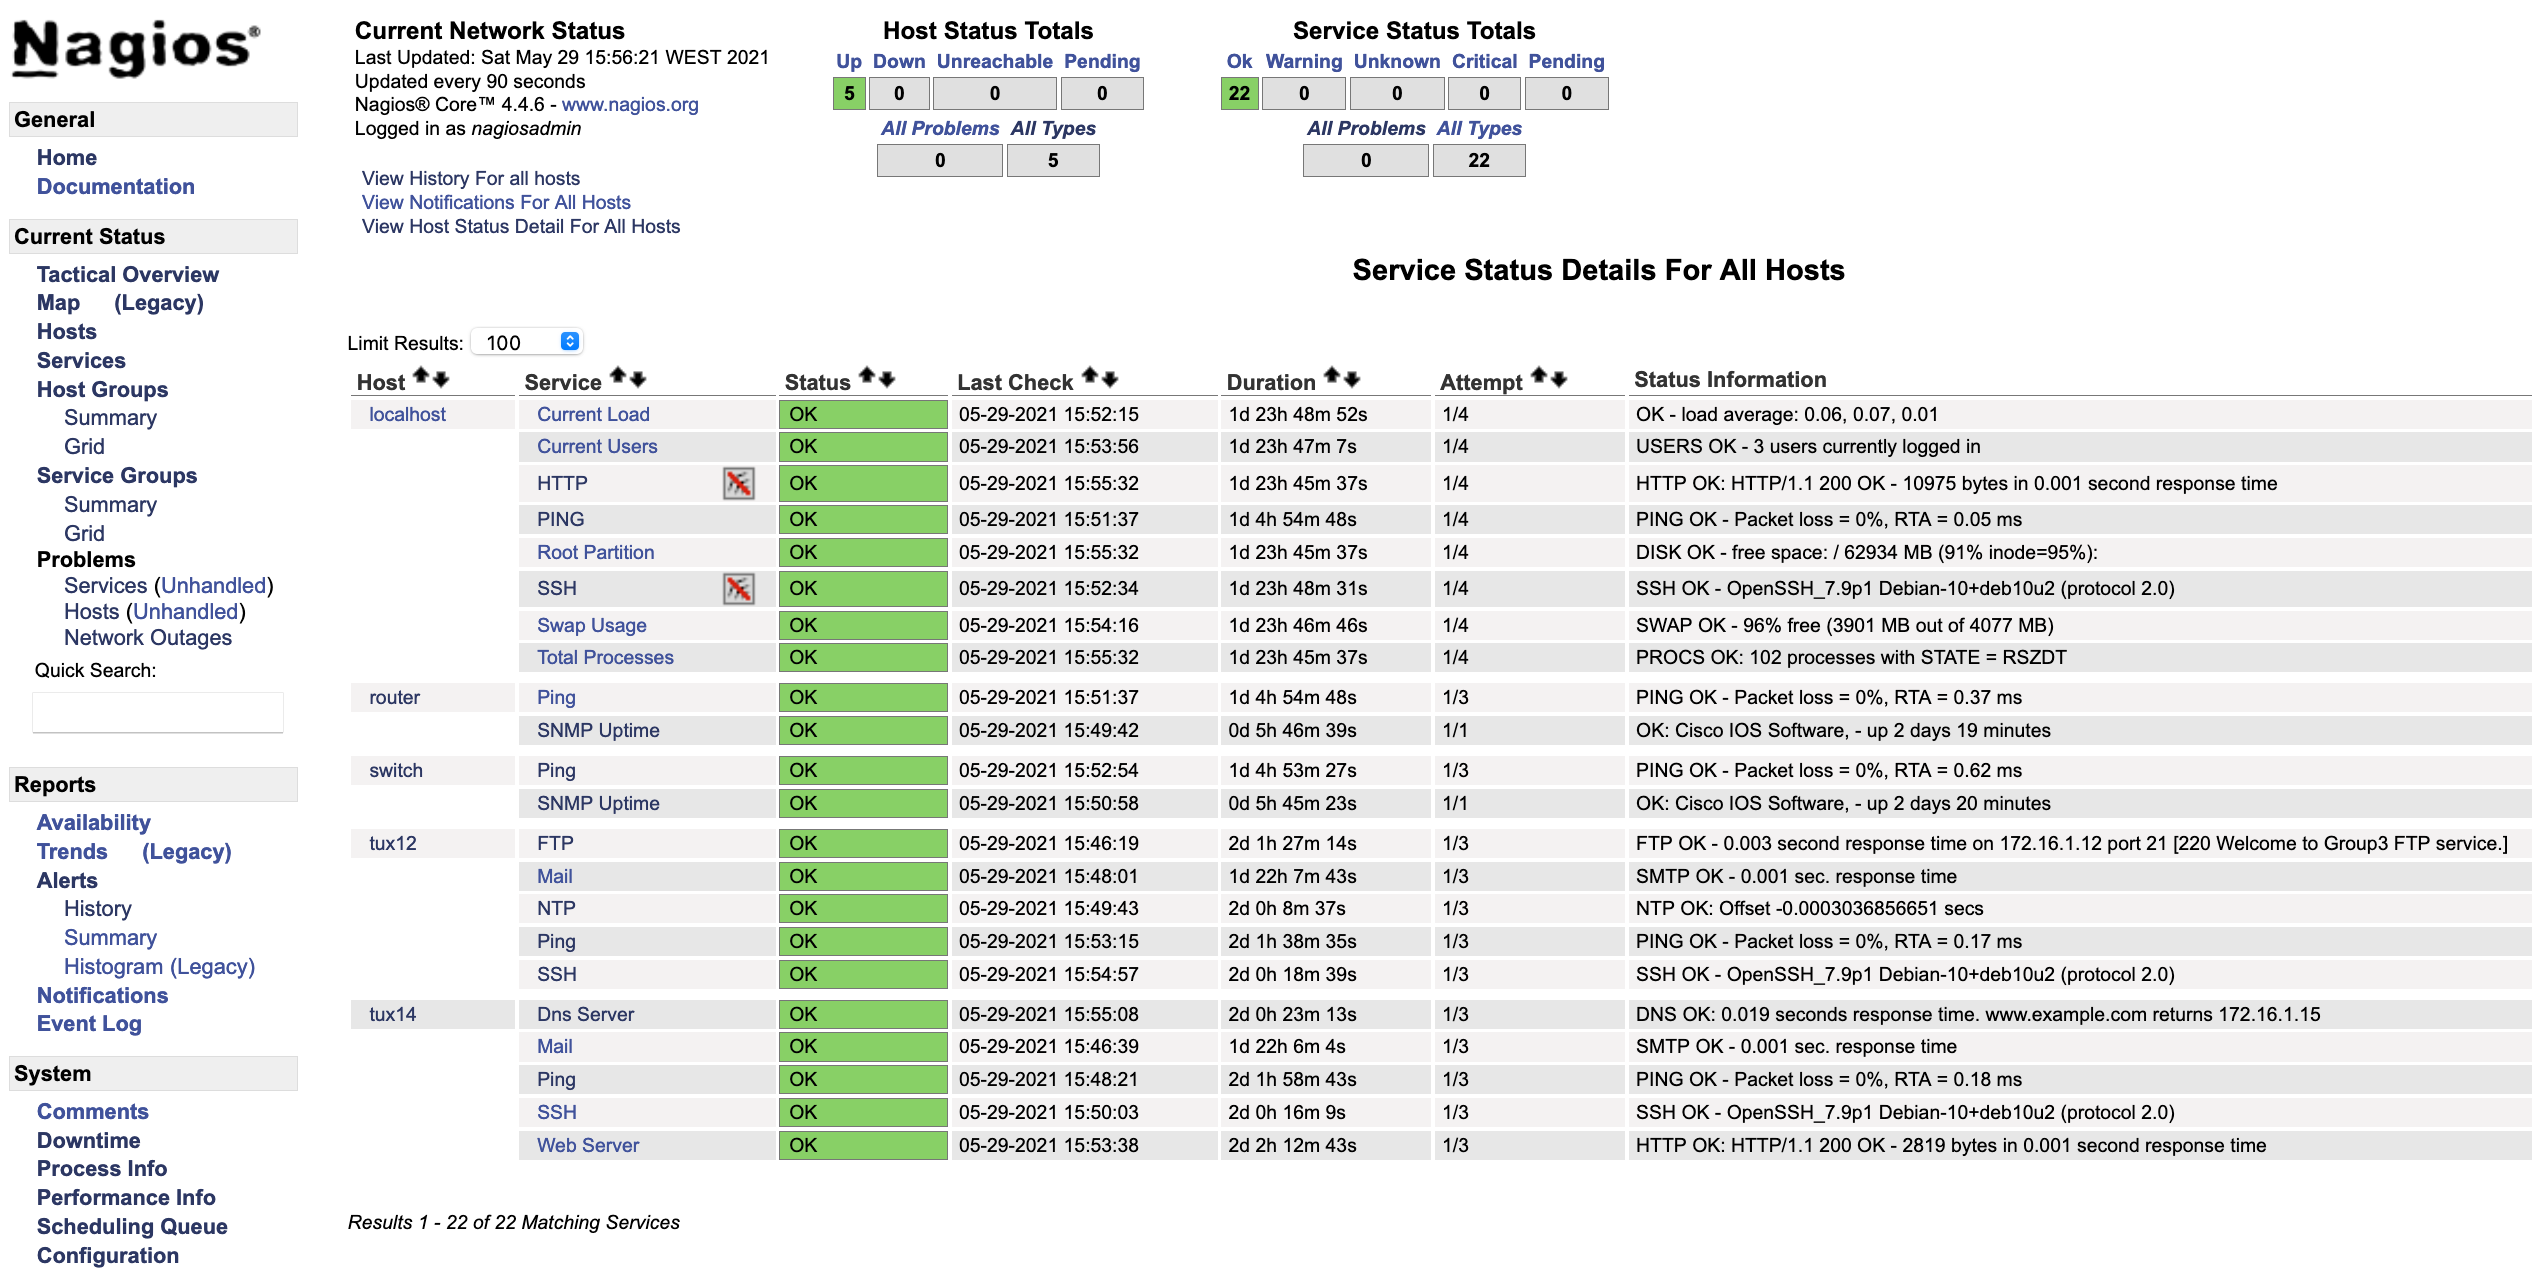
\includegraphics[width=.99\linewidth]{figs/nagios/nagios_web}
    \caption{Interface Web com o status dos serviços e hosts}
    \label{fig:nagios_web}
\end{figure}

Como observado, todos os serviços estão \textbf{OK}.
Também é apresentada informação relativamente ao \textit{uptime} dos serviços, assim como o retorno dos testes.

O campo \textbf{Last Check} indica quando foi executado o último teste.
É possível configurar o Nagios para aumentar a frequência de testes, no entanto isso aumenta também o tráfego interno de controlo pelo que é um \textit{trade-off} a ter em conta.

Clicando em cada serviço ou host, é possível obter informação mais específica.
No entanto, é uma \textit{frontend} bastante simples e intuitiva.

\pagebreak

\section{Teste de falhas}

Primeiramente, simulou-se falhas nos serviços, parando alguns processos nos Tuxs:

\begin{center}
    Tux12 \\
    \verb|systemctl stop vsftpd - Falha do servidor FTP| \\
    \verb|systemctl stop postfix - Falha do servidor Email| \\

    \vspace{1cm}
    Tux14 \\
    \verb|systemctl stop bind9 - Falha do servidor DNS| \\
    \verb|systemctl stop apache2 - Falha do servidor HTTP|
\end{center}

Após algum tempo de atualização de informação, o output da interface do Nagios foi o seguinte:

\begin{figure}[H]
    \centering
    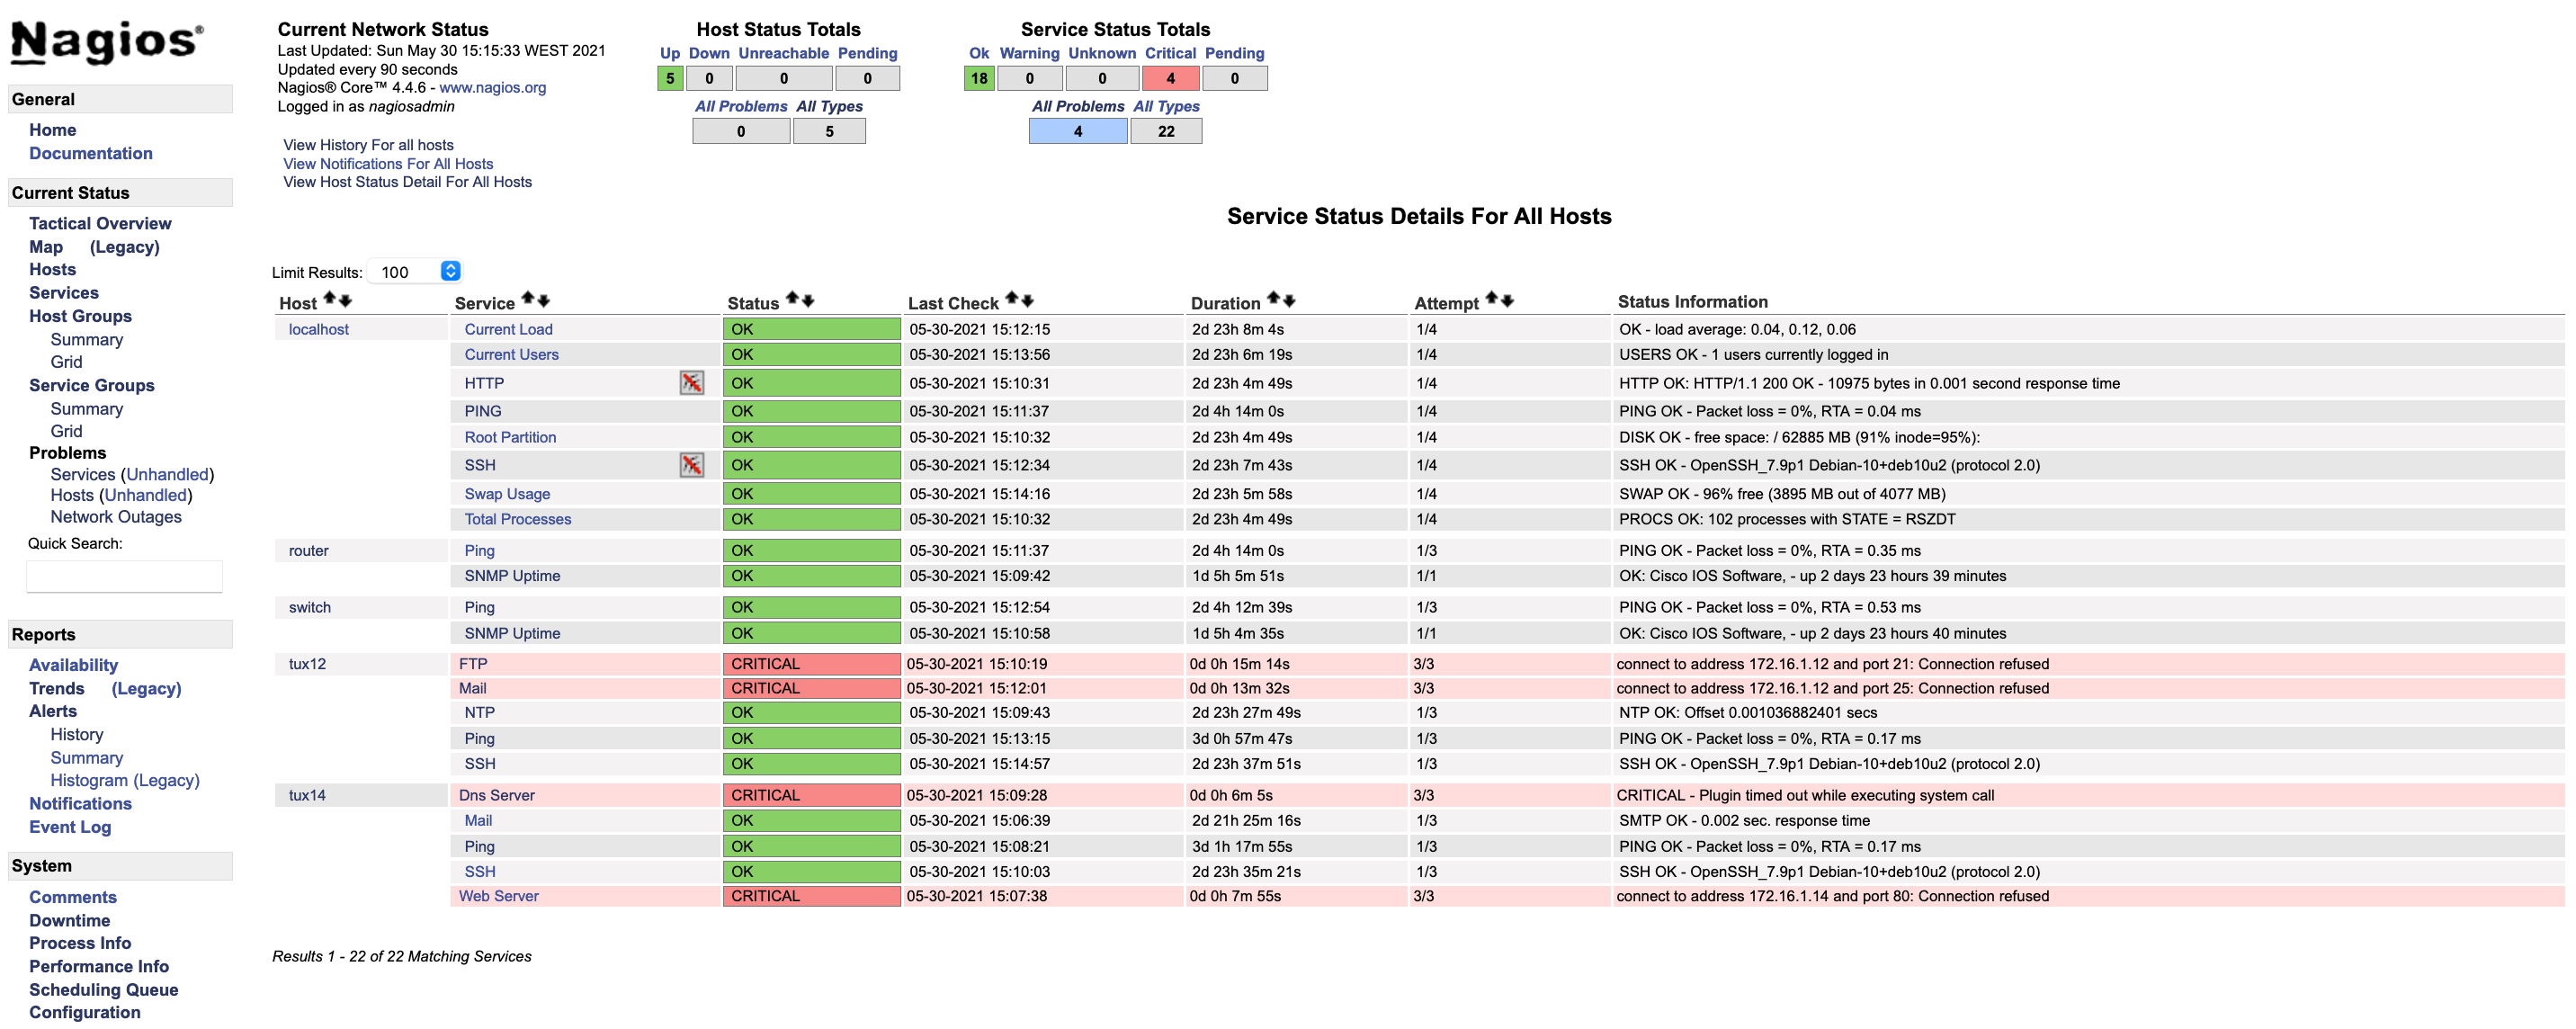
\includegraphics[width=\linewidth]{figs/nagios/nagios_errors}
    \caption{Falha de serviços}
    \label{fig:nagios_errors}
\end{figure}

Como se observa, os serviços desativados estão \textbf{CRITICAL}, sendo possível observar o output dos plugins.
É também apresentado quando tempo já passou desde que o serviço falhou.

De seguida simulou-se uma falha no Tux14.
Para se simular este evento, configurou-se dois \textit{cronjobs} consecutivos:
\begin{itemize}
    \item ifconfig eth0 down: cortar a ligação do Tux14 à rede
    \item ifconfig eth0 up: ativar novamente a interface para retomar o acesso 15 minutos depois do anterior
\end{itemize}

\begin{figure}[H]
    \centering
    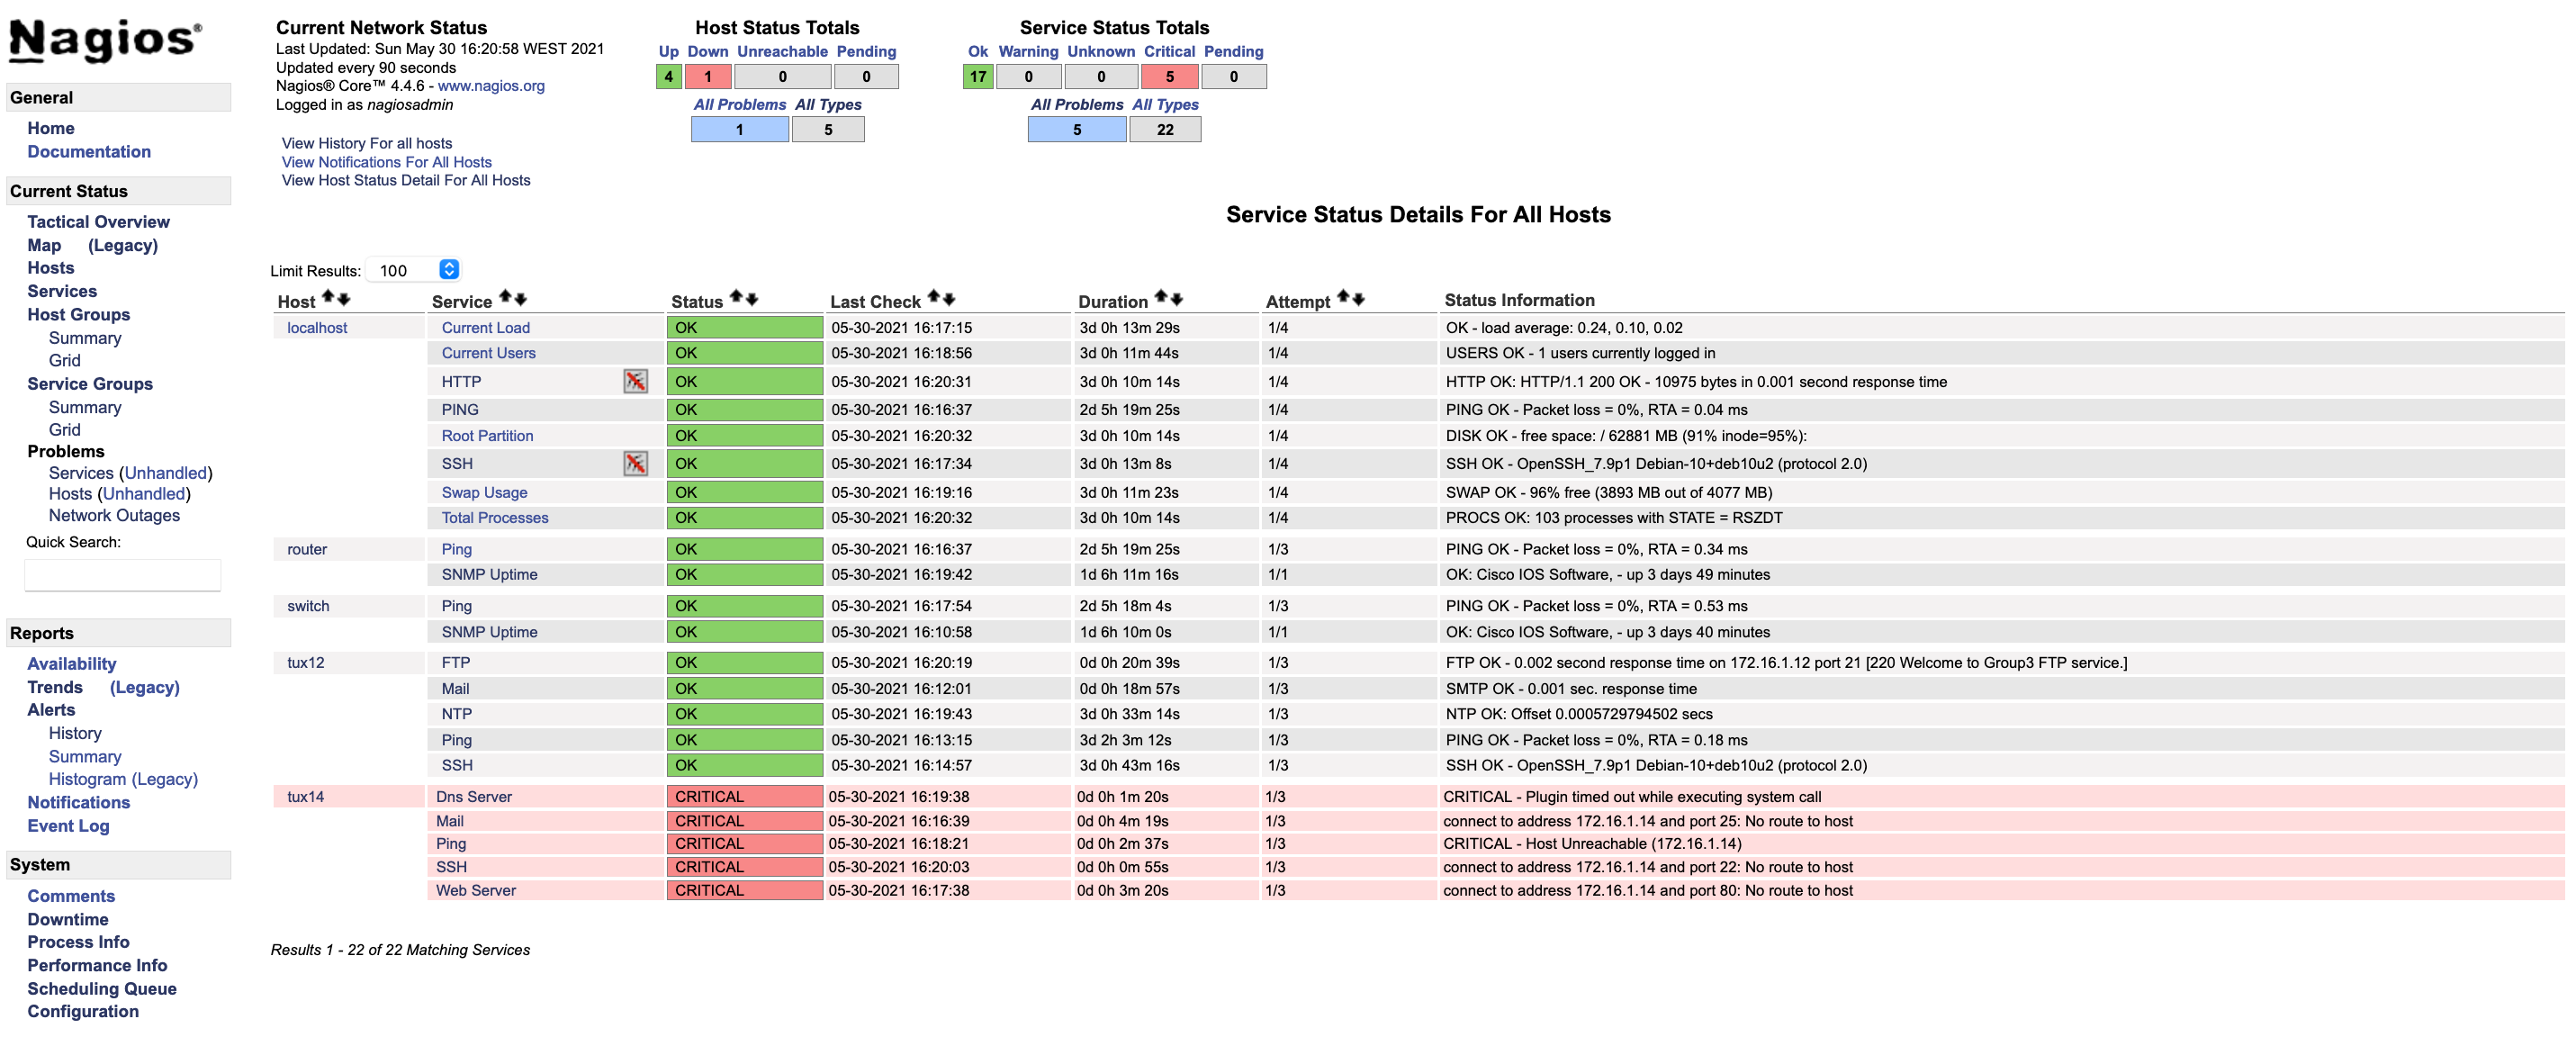
\includegraphics[width=\linewidth]{figs/nagios/nagios_tux14_down}
    \caption{Falha do Tux14}
    \label{fig:nagios_tux14_down}
\end{figure}

Neste cenário, não só estão os serviços no estado \textbf{CRITICAL}, mas também os testes de conectividade Ping e SSH.
O próprio host aparece a vermelho, e no topo da página é possível observar que há um host que está \textit{down}.

O Nagios demorou cerca de 1 minuto a detetar que host estava down, que está relacionado com a frequência do teste configurada.